\documentclass[10pt,twocolumn]{article}
\usepackage[a4paper,top=25mm,bottom=25mm,left=20mm,right=20mm]{geometry}
\usepackage[T1]{fontenc}
\usepackage[utf8]{inputenc}
\usepackage{lmodern,graphicx,amsmath,amssymb,booktabs}
\usepackage[font=small,labelfont=bf]{caption}
\usepackage[hyphens]{url}
\usepackage[hidelinks,breaklinks]{hyperref}
\renewcommand{\rmdefault}{ptm}
\setlength{\columnsep}{0.23in}
\setlength{\emergencystretch}{1.5em}
\renewcommand{\thesection}{\arabic{section}}
\renewcommand{\thesubsection}{\thesection.\arabic{subsection}}
\setlength{\textfloatsep}{8pt plus 2pt minus 2pt}
\setlength{\dbltextfloatsep}{8pt plus 2pt minus 2pt}
\setlength{\intextsep}{6pt plus 2pt minus 2pt}
\captionsetup{skip=3pt}
\renewcommand{\topfraction}{0.95}
\renewcommand{\dbltopfraction}{0.95}
\renewcommand{\textfraction}{0.05}
\renewcommand{\floatpagefraction}{0.8}
\graphicspath{{../figures/2023/}}
\hypersetup{pdftitle={Sentinel-GL: Dependency-Safe Multisensor Masked Autoencoding and Retrospective Anomaly Diagnostics for Himalayan Glacial Lakes},pdfauthor={Aditya Shrestha}}
\title{\vspace{-1.2em}\fontsize{12}{14}\selectfont\bfseries Sentinel-GL: Dependency-Safe Multisensor Masked Autoencoding and Retrospective Anomaly Diagnostics for Himalayan Glacial Lakes}
\author{\fontsize{10.5}{12.5}\selectfont\bfseries Aditya Shrestha$^{1}$\thanks{Corresponding author: Aditya Shrestha, Department of Computer Science and Engineering (DoCSE), School of Engineering, Kathmandu University, Dhulikhel, Nepal. Email: \href{mailto:adityashrestha39@gmail.com}{\nolinkurl{adityashrestha39@gmail.com}} (Institutional: \href{mailto:as03233622@student.ku.edu.np}{\nolinkurl{as03233622@student.ku.edu.np}}). (Received: \hspace{1.0cm} Accepted: to be filled by the Editorial Board)}\\
\small $^1$Department of Computer Science and Engineering (DoCSE), School of Engineering,\\
\small Kathmandu University, Dhulikhel, Nepal}
\date{}
\begin{document}
\fontsize{10.5}{12.0}\selectfont
\raggedbottom
\maketitle
\begin{abstract}
Reliable satellite anomaly analysis requires separating measurement support, deterministic feature dependencies, and developmental model fitting. We assemble 48 Sentinel-2 observations spanning January--November 2023 over South Lhonak and Khangchung Tsho, supplemented by one shared September Sentinel-1 VV/VH product. Source-derived 20-m query grids retain explicit missingness and native radiometric lineage. A 1,062,919-parameter temporal masked autoencoder uses four quadrant folds, optical dependency closure, fitting-only normalization, and five training seeds. Frozen latent and fused scores are compared with Isolation Forest, a one-class SVM, sensor-stratified robust PCA, and CUSUM. All 188 genuinely observed query quadrants per seed are scored; 12 unsupported quadrants remain unavailable. South Lhonak's median reconstruction score changes from 0.0477 before the event to 0.0442 afterward, while latent scores increase at both sites. Thus, reconstruction error does not show a specific post-breach spike in this corpus. Robust PCA converges numerically, but independent warning labels and annual exposure are absent. The findings characterize retrospective surface-anomaly diagnostics, not validated precursors or operational GLOF warning skill.
\end{abstract}
\noindent\textbf{\textit{Keywords:}} Glacial lakes, Sentinel-1, Sentinel-2, masked autoencoders, anomaly detection.

\section{Introduction}
Glacial lake growth and changing exposure motivate satellite monitoring across high mountain regions (Shugar et al., 2020; Zheng et al., 2021; Taylor et al., 2023). The October 2023 South Lhonak disaster illustrates a cascading process whose hazard interpretation requires physical evidence beyond an unusual image score (Sattar et al., 2025). Retrospective satellite detection of lake changes is an established research direction (Veh et al., 2018); consequently, an anomaly detector's contribution cannot be justified solely by applying a transformer to a known event.

A central difficulty is observational dependence. Optical indices reuse the same bands, spatial patches share landscapes and acquisition conditions, and repeated optimization seeds share the same source corpus. Treating those dependencies as independent information can produce an apparently successful model without establishing warning performance. Missing optical observations introduce a further ambiguity: a score trajectory can reflect changing cloud or snow support rather than changing lake conditions. Reviews of time-series anomaly detection also caution that complex learned methods need credible simple comparisons and explicit evaluation assumptions (Sarfraz et al., 2024).

We investigate a bounded, retrospective question: what source-supported reconstruction and fitted anomaly trajectories arise over two fixed Himalayan regions during 2023 when derived-channel leakage, fitting support, sensor missingness, and temporal context are explicitly controlled? South Lhonak is the event-region case; Khangchung Tsho is a regional developmental comparator, not an independently ascertained negative event label. Our contributions are an asynchronous source-bound panel, four-fold dependency-safe reconstruction, fitted latent and fused scoring, sensor-stratified classical comparisons, and an empirical account of their measured behavior and limitations. We make no claim of a new general transformer architecture or validated prospective GLOF forecasting.

\section{Literature}
Optical multispectral monitoring with Sentinel-2 (Drusch et al., 2012) relies on spectral ratios such as NDWI (McFeeters, 1996) and MNDWI (Xu, 2006) to delineate open-water features, while C-band Synthetic Aperture Radar (SAR) from Sentinel-1 provides cloud-penetrating backscatter observations (Torres et al., 2012). In multivariate time-series representation learning, transformer encoders (Vaswani et al., 2017; Zerveas et al., 2021) and masked autoencoders (He et al., 2022) learn contextual representations by reconstructing masked inputs. However, critical reviews of unsupervised time-series anomaly detection caution that deep architectures require transparent comparisons against classical detectors such as Isolation Forest (Liu et al., 2008), One-Class SVM (Sch\"olkopf et al., 2001), Robust PCA (Cand\`es et al., 2009; Lin et al., 2010), and CUSUM (Page, 1954), as well as extreme-value threshold calibration (Pickands, 1975; Davison and Smith, 1990) free of evaluation leakage (Sarfraz et al., 2024).

\section{Methods and Procedures}
\subsection{Spatial and temporal design}
We fix query centroids at $(27.915^\circ\mathrm{N},88.204^\circ\mathrm{E})$ for South Lhonak and $(27.985^\circ\mathrm{N},88.752^\circ\mathrm{E})$ for Khangchung Tsho. Each region uses an integer-aligned $499\times499$ grid in EPSG:32645 with 20-m pixels. Its side length is 9.98 km and its area is 99.6004 km$^2$. These grids include surrounding terrain and are not lake polygons; ROI-wide statistics must not be interpreted as lake-only measurements.

The optical acquisition window is 1 January--15 November 2023. Within 24 equal-duration temporal bins per site, acquisition selection uses the lowest catalogue scene cloud fraction, then acquisition time and product identity. Selection precedes model scoring. Full projected tile coverage is required; point intersection alone is insufficient near a tile edge. The resulting sequence contains 24 Sentinel-2 observations per site, including pre-monsoon, monsoon, and post-event dates. Scene cloud metadata guides acquisition selection; the actual ROI clear fraction is computed independently from source classification pixels (Fig.~\ref{fig:timeline}).

\begin{figure*}[t]
\centering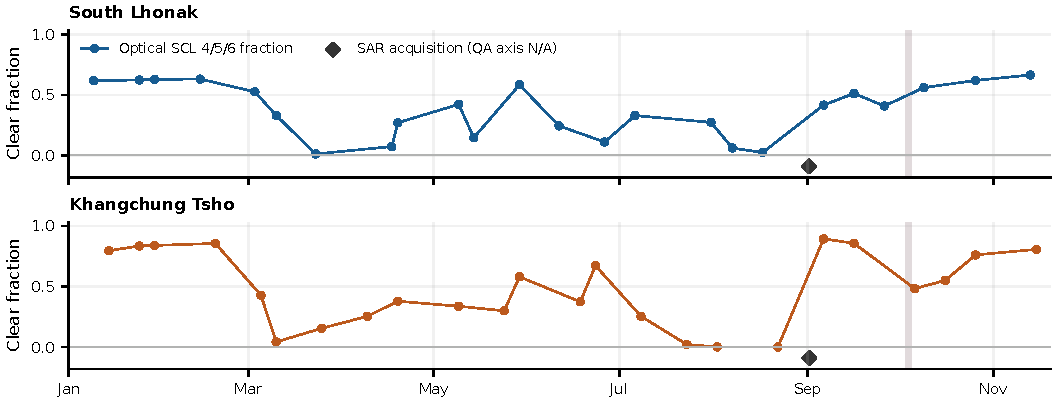
\includegraphics[width=\textwidth]{fig1_observation_timeline.pdf}
\caption{Source-supported 2023 observation sequence. Optical points show the fraction of the fixed ROI assigned SCL 4/5/6; connected points are measured acquisitions, not interpolated daily inputs. Diamonds indicate the single retained 1 September SAR acquisition at both sites, with no optical clear-fraction meaning. The 3--4 October event bracket is shaded. Zero clear support remains an observed acquisition with no usable optical model targets.}
\label{fig:timeline}
\end{figure*}

A single ascending Sentinel-1 IW GRD VV/VH product from 1 September covers both sites. Additional same-orbit acquisitions were requested, but the authenticated provider returned an expired-token response before a new archive was transferred. Thus, 50 site--sensor observations correspond to 49 unique provider products. The SAR observation provides a genuine asynchronous modality but cannot establish a SAR temporal response to the breach. Acquisition timestamps provide retrospective ordering; historical operational delivery availability is not independently reconstructed.

\subsection{Optical radiometry and explicit QA}
Sentinel-2 supplies complementary visible, near-infrared and shortwave-infrared observations (Drusch et al., 2012). We read B03, B08, B11 and scene classification from cloud-optimized assets through bounded HTTP byte ranges. Exact received-range SHA-256 digests, catalogue identities, declared full-object checksums, native product/granule metadata, and derived ROI hashes are retained. A partial-range digest does not verify the whole remote COG. Processing baselines 05.09, 05.10 and 05.11 are recorded per granule, rather than treated as interchangeable versions without radiometric checks.

For source digital number $d$, BOA reflectance is $\rho=(d+o)/Q$, using native band-specific additive offset $o$ and quantification value $Q$. Scale and offset are applied once, checked against metadata. B03 and B08 are reduced from 10 m by an exact aligned $2\times2$ arithmetic mean requiring all four native pixels; B11 and SCL use native 20-m support. Optical validity additionally requires SCL 4, 5 or 6. Invalid values remain NaN behind false validity masks.

We calculate NDWI (McFeeters, 1996) and MNDWI (Xu, 2006):
\begin{equation}
 I_N=\frac{\rho_3-\rho_8}{\rho_3+\rho_8},\qquad
 I_M=\frac{\rho_3-\rho_{11}}{\rho_3+\rho_{11}}.
\end{equation}
Each index requires both source bands and a finite, nonzero denominator. Independent replay uses the exact stored reflectances with float64 arithmetic followed by the declared float32 serialization. Signed BOA reflectance can produce ratios outside $[-1,1]$ near small denominators; those values are retained rather than epsilon-clamped. An $I_N>0$ and $I_M>0$ mask is a candidate spectral indicator only. Without independent snow/ice and shoreline validation, its area is not a lake-area estimate.

\subsection{Native SAR calibration and geometry}
Sentinel-1 provides microwave observations complementary to optical support (Torres et al., 2012). Native measurement and annotation identities are joined across VV/VH, calibration, noise, and acquisition metadata. Native timestamps are normalized to UTC using the Sentinel product convention and checked against the exact catalogue product interval. Calibration uses a bounded native line/sample window enclosing each target ROI, with LUT support respected and no extrapolated noise values.

Writing $A_\sigma$ for the interpolated sigma-nought calibration LUT, $N_R$ and $N_A$ for native range and azimuth noise terms, the retained radiometric variants are
\begin{align}
 \sigma^0_{r}&=\frac{d^2}{A_\sigma^2},&
 \mathrm{NESZ}&=\frac{N_RN_A}{A_\sigma^2},\\
 \sigma^0_{s}&=\frac{d^2-N_RN_A}{A_\sigma^2}.
\end{align}
The signed variant is not clipped at zero. $10\log_{10}(\sigma^0)$ is defined only on strictly positive valid support. Linear-power resampling precedes dB conversion, with explicit valid bilinear weights. Model channels use raw linear VV/VH; signed-noise and NESZ arrays remain separately identified diagnostics.

Target-grid SAR geometry comes from annotation ellipsoid tiepoint inversion, without DEM terrain correction, terrain flattening, or a measured cross-sensor registration error. Spatially aligned array dimensions therefore do not prove terrain-corrected shoreline registration. Figure~\ref{fig:spatial} separates the optical pre/post comparison from the single-date SAR distributions.

\begin{figure*}[t]
\centering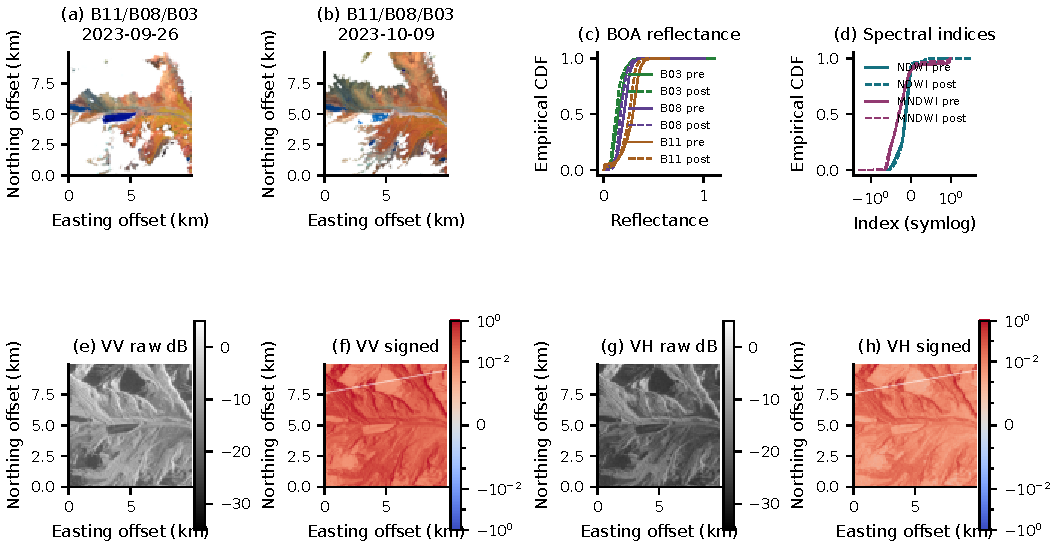
\includegraphics[width=\textwidth]{fig2_source_distributions.pdf}
\caption{South Lhonak source diagnostics. (a,b) Nearest selected pre/post optical acquisitions, 26 September and 9 October, shown as B11/B08/B03 false color with common reflectance display scale $[0,0.4]$; white indicates excluded QA. (c,d) ROI empirical distributions of the three bands and two indices, with solid pre-event and dashed post-event curves; the index axis is symmetric-logarithmic. (e--h) Raw dB and signed linear VV/VH from 1 September only, on ellipsoid tiepoint geometry. Signed noise-support gaps remain missing. Color normalization affects display only. These are query-ROI measurements, not validated water-only or terrain-corrected comparisons.}
\label{fig:spatial}
\end{figure*}

\subsection{Fitting support and asynchronous tokens}
For raster row $r$ and column $c$, define the spatial parity
\begin{equation}
 P(r,c)=\left(\left\lfloor r/16\right\rfloor+\left\lfloor c/16\right\rfloor\right)\bmod 2.
\end{equation}
Parity 0 supplies fitting pixels; parity 1 supplies development monitoring. Fitting and checkpoint selection use only acquisitions ending strictly before 2 October 2023, 18:30 UTC (the start of 3 October in Nepal). Post-event observations cannot fit the normalizer, encoder, reference bank or score standardizers. Shared scenes and neighboring checkerboard cells remain spatially dependent: the split prevents direct pixel reuse but does not create independent physical replication.

Per-channel float64 Welford accumulation (Welford, 1962) estimates the fitting mean and population variance from genuine parity-0 support. The frozen transform is applied without recomputing monitor statistics. Channels with unavailable or zero-variance fitting support remain explicitly unavailable. Each acquisition produces four quadrant tokens, each pooling only valid pixels of its own sensor and parity. Denominators retain the actual source-pixel support. Optical and SAR groups are separate asynchronous arrivals; absent sensor channels, cloud gaps, weather and DEM remain unobserved. No temporal interpolation or synthetic measurement enters tokens or targets.

For a query at acquisition time $t$, context contains only same-site arrivals at times $\leq t$. This is a causal \emph{input context}, not a prospective training experiment: fitted parameters use the declared whole pre-breach period, including dates later than early-period queries. All pre-period trajectories are consequently development-exposed retrospective reconstructions. Khangchung and South Lhonak also share one SAR product; model seeds are repeated optimizations conditional on this corpus, not independent lake samples. Physical sampling dependencies and fitted-model provenance have distinct interpretations.

\subsection{Masking and autoencoder}
Transformers (Vaswani et al., 2017), masked autoencoders (He et al., 2022), and time-series representation learning (Zerveas et al., 2021) motivate the model, without implying a general architectural novelty claim. The encoder dimension is 128 with four attention heads and four layers; the decoder has two layers. Separate sensor projections incorporate observed-channel masks, followed by modality, quadrant and continuous day-of-year/elapsed-time identities. Target decoder tokens retain their identities but never their hidden measurements.

For each query, four separate folds hide quadrants $q=0,1,2,3$ in turn. Only genuinely observed target channels contribute to loss; a completely unobserved quadrant correctly remains unscored. Hiding every observed quadrant in its own fold removes the earlier one-quadrant coverage limitation without inventing support. Remaining same-date quadrants and earlier acquisitions provide context.

Optical dependency closure hides all five optical channels of a targeted token. Otherwise, for example,
\begin{equation}
 \rho_3=\rho_8\frac{1+I_N}{1-I_N}
\end{equation}
can algebraically reveal a supposedly hidden band on its defined domain. Masking a band while exposing its deterministic index would be target leakage. For target set $T_q$, the reconstruction score is
\begin{equation}
 A(t)=\frac{\sum_q\sum_{j\in T_q}(\hat z_{qj}-z_{qj})^2}{\sum_q |T_q|},
\end{equation}
with an explicit unavailable result when the denominator is zero. This averages supported quadrant-channel targets, not independent events or every image pixel as separate cases.

Five seeds use deterministic CPU execution and AdamW (Loshchilov and Hutter, 2019), learning rate $3\times10^{-4}$, weight decay $10^{-4}$, two warmup epochs, and gradient clipping at 1. The prospective maximum is 80 epochs, with checkpoint eligibility and minimum training at epoch 12, patience 12 eligible nonimprovements, and improvement tolerance $10^{-4}$. Selection minimizes parity-1 masked MSE on pre-breach development scenes. Selected checkpoints are reloaded and their losses replayed. A plateau or exhausted budget is an optimization observation, not proof of a global optimum.

\begin{figure*}[t]
\centering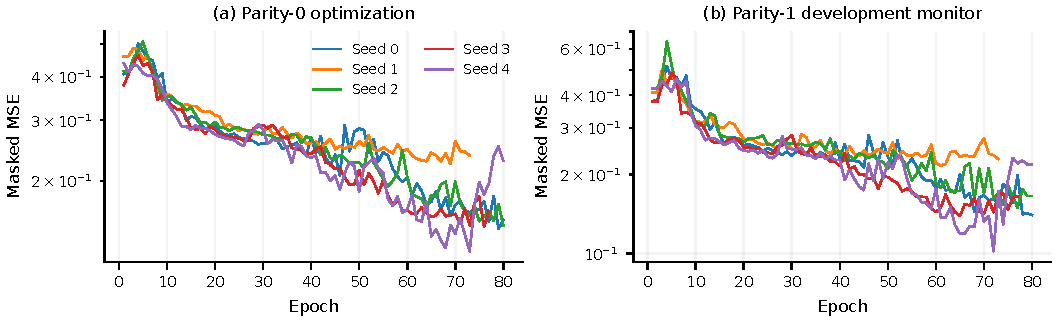
\includegraphics[width=\textwidth]{fig3_optimization.pdf}
\caption{Recorded five-seed optimization histories. Left: parity-0 masked training loss during parameter updates. Right: parity-1 masked development loss on the same pre-breach scenes. Logarithmic axes retain the measured scale. Checkpoint selection uses only eligible pre-breach development evaluations; seed variation does not quantify population uncertainty.}
\label{fig:training}
\end{figure*}

\subsection{Latent and fused scores}
Frozen selected encoders supply visible, non-target embeddings for a parity-0 fitting reference. Within each site and sensor, an eight-component PCA and five-neighbor distance reference define score $B$. Neighbor distances are reduced by distinct acquisition, excluding the query's own provider product or same-sensor timestamp. These exclusions prevent duplicate quadrants of the same scene from acting as independent neighbors. A sensor with insufficient distinct fitting acquisitions has an unavailable latent score, even if it has many spatial pixels.

The prospectively fixed fused score is
\begin{equation}
 C=\tfrac12(A-\mu_A)/s_A+\tfrac12(B-\mu_B)/s_B,
\end{equation}
where all standardizers use parity-0 pre-breach fitting scores. Parity-1 scores do not fit these statistics. Missing components or degenerate scales produce an unavailable fused score, rather than a substituted zero. This fitted scaling permits a declared combination; it does not make scores calibrated event probabilities.

\subsection{Classical comparisons and sequential diagnostics}
Isolation Forest (Liu et al., 2008) uses 100 trees and observed-feature support, with proportional subtree routing where applicable. A one-class SVM (Sch\"olkopf et al., 2001) uses a positive-semidefinite RBF construction and $\nu=0.1$. Both fit only declared parity-0 pre-breach rows and score parity-1 rows throughout the sequence. Models are stratified by sensor, avoiding a disconnected seven-channel matrix whose optical and SAR rows never observe the other modality.

Robust PCA (Cand\`es et al., 2009) is fitted with an augmented-Lagrangian splitting method (Lin et al., 2010) separately on optical five-channel and SAR two-channel matrices, with maximum 1000 iterations and tolerance $10^{-5}$. For complete observed matrices, fixed-penalty ADMM uses $\lambda=1/\sqrt{\max(m,n)}$, $\mu=5/\|D\|_2$, and a dual-feasible initialization. Wholly unsupported rows are excluded from the objective, not filled. Both normalized primal and dual residuals must meet tolerance; subgradient KKT residuals are also recorded. Actual residuals and rank determine the reported status. Monitor scores are subspace residuals; nonconvergence cannot be repaired by relabeling a decomposition as converged.

A two-sided CUSUM (Page, 1954) processes chronological site--sensor Isolation Forest scores, centered and scaled by fitting scores. Its reference allowance is 0.5; unavailable scores or gaps exceeding 90 days reset accumulation. It is a descriptive cumulative-change trace, with no calibrated warning threshold. Peaks-over-threshold/GPD theory (Pickands, 1975; Davison and Smith, 1990) requires justified exceedances and exposure. A two-ROI development sequence without an independently verified opportunity schedule cannot establish one false alarm per lake-year. Such annual calibration and detection-performance quantities remain unavailable.

\section{Empirical Results}
\subsection{Source support and optimization}
The retained optical clear fractions range from 1.27\% to 66.46\% at South Lhonak (median 41.17\%) and from 0 to 89.25\% at Khangchung Tsho (median 45.50\%). One comparator acquisition has no valid optical targets. Table~\ref{tab:corpus} distinguishes acquisition counts from usable score support; the two SAR rows share one product and one date.

\begin{table}[t]\centering\small
\caption{Recorded observation support. Optical pre/post counts denote acquisitions; the comparator has one wholly unsupported pre-period image.}\label{tab:corpus}
\begin{tabular}{lrrr}\toprule
Region & Optical pre & Optical post & SAR dates\\\midrule
South Lhonak & 21 & 3 & 1\\
Khangchung Tsho & 20 & 4 & 1\\\bottomrule
\end{tabular}
\end{table}

The model has 1,062,919 trainable parameters. Fitting membership contains 43 site--sensor observations, of which 42 supply reconstruction targets. Every seed scores all 188 observed parity-1 quadrants; the other 12 of 200 possible quadrants lack genuine source support. This yields 49 acquisition-level reconstruction scores per seed, not 50 fabricated complete rows. Five-seed selected development losses range from 0.101839 to 0.215871 (Table~\ref{tab:seeds}, Fig.~\ref{fig:training}). All selected-checkpoint replay differences are exactly zero. Three runs reach the 80-epoch budget; two stop by the prescribed patience rule. Neither stopping condition proves global convergence.

\begin{table}[t]\centering\small
\caption{Actual selected-checkpoint evidence. Development MSE uses parity-1 pixels of pre-breach scenes.}\label{tab:seeds}
\begin{tabular}{rrrr}\toprule
Seed & Epochs run & Selected epoch & Monitor MSE\\\midrule
0 & 80 & 80 & 0.140137\\
1 & 73 & 61 & 0.215871\\
2 & 80 & 77 & 0.149476\\
3 & 77 & 65 & 0.138823\\
4 & 80 & 72 & 0.101839\\
\bottomrule\end{tabular}
\end{table}

\subsection{Retrospective score contrasts}
Table~\ref{tab:contrasts} first takes the median across training seeds at each acquisition for learned scores, then the median across acquisitions within the pre/post period. Baseline medians use their single fixed fit. There are 21 usable pre-event and 3 post-event optical acquisitions at South Lhonak, versus 19 and 4 at Khangchung. These are descriptive temporal summaries; acquisitions and seeds are not pooled as independent event replicates.

\begin{table}[t]\centering\scriptsize
\caption{Optical acquisition-level medians, by method's own units. SL: South Lhonak; KT: Khangchung Tsho. No column is a detection-performance metric.}\label{tab:contrasts}
\begin{tabular}{lrrrr}\toprule
Method & SL pre & SL post & KT pre & KT post\\\midrule
T-MAE A & 0.0477 & 0.0442 & 0.0359 & 0.0244\\
T-MAE B & 1.0086 & 3.1894 & 1.3871 & 2.9591\\
T-MAE C & -0.3062 & 0.2853 & -0.3217 & 0.0454\\
Isolation Forest & 0.4277 & 0.4890 & 0.4189 & 0.4476\\
One-Class SVM & -0.1898 & 0.0394 & -0.1897 & -0.0396\\
RPCA residual & 0.0515 & 0.0368 & 0.0427 & 0.0324\\
CUSUM & 0.0000 & 0.2171 & 0.0000 & 0.0000\\
\bottomrule\end{tabular}
\end{table}

South Lhonak's reconstruction median decreases from 0.0477 to 0.0442; the comparator decreases from 0.0359 to 0.0244. Reconstruction therefore provides no distinctive post-breach increase under this representation. Latent-distance medians increase from 1.0086 to 3.1894 at South Lhonak and from 1.3871 to 2.9591 at the comparator. Elevated latent values are also present before October: September medians are 4.4797 and 2.9420, respectively. Thus, the latent shift is not uniquely localized to the known breach. Fused scores combine these differing signals rather than independently confirming an event mechanism. Seed ranges in Fig.~\ref{fig:scores} further show optimization-dependent variation.

The first selected post-event optical images occur on 9 October at South Lhonak and 6 October at Khangchung. Surface changes visible in the South Lhonak pre/post image pair do not imply that an ROI-wide learned reconstruction score must increase: spatial pooling, varying clear support, seasonal terrain conditions and the fitting objective affect that score. These results do not establish a precursor signal; the entire pre-period informed the fitted states.

\subsection{Baseline convergence and estimability}
The optical robust-PCA fit uses 40 source-supported five-channel rows; the wholly unsupported row contributes no objective terms and remains a null query. Its fixed-penalty solver converges in 413 iterations at rank 3, with normalized primal residual $9.9450\times10^{-6}$ and dual residual $1.4947\times10^{-6}$. The largest reported nontrivial subgradient/dual-feasibility violation is below $7\times10^{-6}$. The two-row SAR fit converges in 1 iteration at rank 1; this is numerical convergence on one shared date, not temporal validation. Optical monitor residuals remain computed on parity-1 support throughout.

The final record contains 950 method--seed--observation rows. Optical latent and fused scores are available where source support exists, while SAR latent/fused values are unavailable because one acquisition per site cannot supply five distinct reference acquisitions. Annual POT thresholds, calibrated false-alarm burden, precision--recall, AUROC and warning lead time remain unavailable. CUSUM traces have no validated alarm threshold. Representative attention in Fig.~\ref{fig:attention} demonstrates the fitted computation's internal distributions and cannot establish a causal precursor explanation.


\begin{figure*}[t]
\centering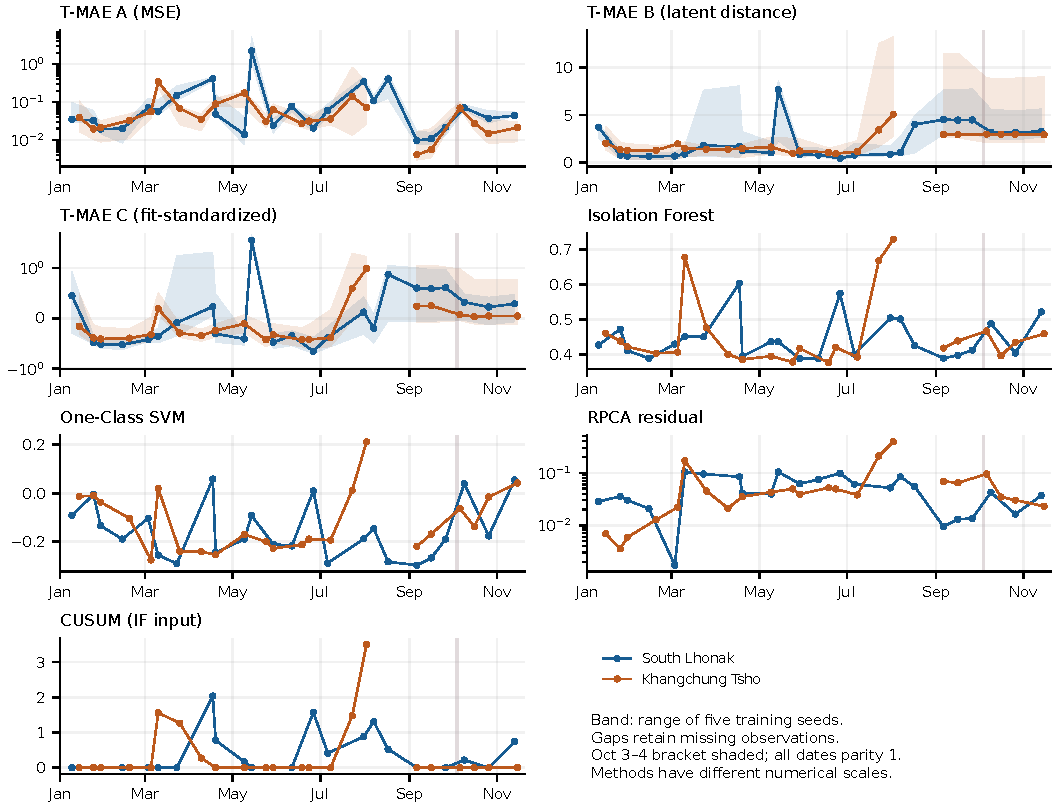
\includegraphics[width=\textwidth]{fig4_anomaly_trajectories.pdf}
\caption{Optical acquisition-level parity-1 trajectories across each site's actual acquisitions. Methods use the same recorded observation sequence. Each method retains its own numerical scale; reconstruction, latent distance, fused score, isolation score, SVM margin, RPCA residual and CUSUM are not interchangeable performance metrics. Learned-score lines are five-seed medians with min--max bands. Missing observations remain breaks. The event bracket is shaded. Pre-breach curves are development-exposed because fitting uses the whole declared pre-breach period; post-event points are excluded from fitting.}
\label{fig:scores}
\end{figure*}

\begin{figure*}[t]
\centering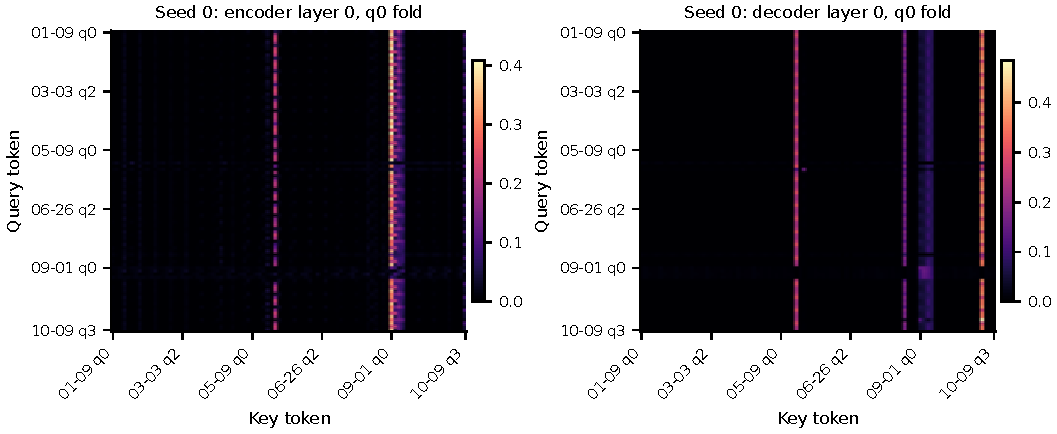
\includegraphics[width=\textwidth]{fig5_attention.pdf}
\caption{Representative seed-0 internal attention for the first source-supported post-event South Lhonak optical query, selected by acquisition time rather than score. The first encoder and decoder layers are shown for the q0 masking fold, averaged over four heads in float64. Axes bind to chronological acquisition/quadrant tokens; hidden and naturally absent keys retain their model masks. Attention is an internal learned distribution, not a causal explanation, lake-instability attribution, or independent validation.}
\label{fig:attention}
\end{figure*}

\section{Interpretation and Limitations}
The interpretation is deliberately narrower than a warning-system claim. An optical surface-change score can reflect lake drainage, sediment exposure, seasonal snow, clouds, viewing conditions, or changing valid-pixel composition. Whole-ROI pooling further mixes the lake with substantial surrounding terrain. The pre/post images show observations at different acquisition times and QA masks; they are not a controlled causal intervention. An event-region anomaly that does not exceed the comparator's variation, or an absent precursor signal, remains a substantive negative or inconclusive finding.

The corpus contains two chosen developmental ROIs and one known breach cascade. Its catalogue selection is score-blind but conditions on scene cloud metadata and full tile coverage; it is not an exhaustive, randomly sampled monitoring stream. Optical support changes markedly by season, including acquisitions with no clear comparator pixels. Signed reflectance ratios can be unstable near zero denominators, and retaining them exposes this numerical limitation rather than disguising it. Independent shoreline masks, snow/ice discrimination and QA-stratified sensitivity would be needed to isolate a lake-specific mechanism.

The spatial firewall prevents direct reuse of monitor pixels in the fitted scaler and training loss. It does not remove autocorrelation across neighboring parity cells or common atmosphere, source imagery, terrain and product processing. Hyperparameters and checkpoints are selected within this developmental setting; five seeds do not constitute five independent experiments on nature. Pre-period parameter exposure prevents a confirmatory precursor claim. No independently verified control-event history or representative event cohort supports precision--recall, AUROC, warning lead-time or regional sensitivity estimates.

The asynchronous model combines optical history with only one SAR date, and the raw-linear SAR inputs are not the signed-denoised variant. Additional SAR timing, terrain correction, layover/shadow analysis, and measured cross-sensor alignment are needed before attributing learned cross-modal structure to lake physics. Weather and DEM are absent, not inferred from coordinates. UTC binding establishes timestamp semantics; it does not establish that a product was available to a real-time operator at that instant.

Finally, hashes bind files rather than scientific truth. We retain provider identities, native radiometry, exact HTTP-range receipts, input/output digests, fitted-state membership, selected checkpoints and score components so the numerical path can be inspected. Local unit tests and loss replay establish their specific engineering contracts, not peer-reviewed scientific validity or a portable installation on another platform. The present analysis supplies a reproducible retrospective case study and clear failure boundaries for subsequent independent validation.

\section{Conclusion}
Sentinel-GL combines source-derived 2023 optical observations and native SAR calibration with explicit missingness, dependency-safe quadrant reconstruction, frozen latent/fused scoring, and sensor-stratified comparisons. The empirical results characterize surface-anomaly diagnostics within two developmental ROIs. They do not establish prospective GLOF warning skill. The next scientific test requires independently validated geometry, additional SAR dates, a frozen temporal protocol, and event/control support beyond this development corpus.

\section*{Acknowledgement}
The research was conducted independently without institutional or external grant funding. The institutional affiliation identifies the author's academic affiliation and does not imply institutional sponsorship or endorsement. AI tools assisted with coding, literature organization, verification scripting and manuscript drafting under the author's architectural direction. Aditya Shrestha retains sole responsibility for technical review, intellectual decisions, source verification, interpretation and the submitted content. No AI system is an author. No operational civil-defense use is claimed.

\section*{References}
{\small\begin{list}{}{\setlength{\leftmargin}{1.4em}\setlength{\itemindent}{-1.4em}\setlength{\itemsep}{1.5pt}\setlength{\parsep}{0pt}\setlength{\topsep}{2pt}}
\item Cand\`es, E.J., Li, X., Ma, Y. \& Wright, J. (2009). Robust principal component analysis? \textit{arXiv:0912.3599}.
\item Davison, A.C. \& Smith, R.L. (1990). Models for exceedances over high thresholds. \textit{Journal of the Royal Statistical Society: Series B}, 52(3), 393--425.
\item Drusch, M., Del Bello, U., Carlier, S. \textit{et al.} (2012). Sentinel-2: ESA's optical high-resolution mission for GMES operational services. \textit{Remote Sensing of Environment}, 120, 25--36.
\item He, K., Chen, X., Xie, S., Li, Y., Doll\"ar, P. \& Girshick, R. (2022). Masked autoencoders are scalable vision learners. \textit{Proc. of the IEEE/CVF Conf. on Computer Vision and Pattern Recognition}, 16000--16009.
\item Lin, Z., Chen, M. \& Ma, Y. (2010). The augmented Lagrange multiplier method for exact recovery of corrupted low-rank matrices. \textit{arXiv:1009.5055}.
\item Liu, F.T., Ting, K.M. \& Zhou, Z.H. (2008). Isolation forest. \textit{Proc. of 8th IEEE International Conf. on Data Mining}, 413--422.
\item Loshchilov, I. \& Hutter, F. (2019). Decoupled weight decay regularization. \textit{Proc. of International Conf. on Learning Representations}.
\item McFeeters, S.K. (1996). The use of the Normalized Difference Water Index (NDWI) in the delineation of open water features. \textit{International Journal of Remote Sensing}, 17(7), 1425--1432.
\item Page, E.S. (1954). Continuous inspection schemes. \textit{Biometrika}, 41(1--2), 100--115.
\item Pickands, J. (1975). Statistical inference using extreme order statistics. \textit{The Annals of Statistics}, 3(1), 119--131.
\item Sarfraz, M.S., Chen, M.Y., Layer, L., Peng, K. \& Koulakis, M. (2024). Position: Quo vadis, unsupervised time series anomaly detection? \textit{Proc. of 41st International Conf. on Machine Learning}, 235, 43461--43476.
\item Sattar, A., Cook, K.L., Rai, S.K. \textit{et al.} (2025). The Sikkim flood of October 2023: Drivers, causes, and impacts of a multihazard cascade. \textit{Science}, 387, eads2659.
\item Sch\"olkopf, B., Platt, J.C., Shawe-Taylor, J., Smola, A.J. \& Williamson, R.C. (2001). Estimating the support of a high-dimensional distribution. \textit{Neural Computation}, 13(7), 1443--1471.
\item Shugar, D.H., Burr, A., Haritashya, U.K. \textit{et al.} (2020). Rapid worldwide growth of glacial lakes since 1990. \textit{Nature Climate Change}, 10, 939--945.
\item Taylor, C., Robinson, T.R., Dunning, S., Carr, J.R. \& Westoby, M. (2023). Glacial lake outburst floods threaten millions globally. \textit{Nature Communications}, 14, 487.
\item Torres, R., Snoeij, P., Geudtner, D. \textit{et al.} (2012). GMES Sentinel-1 mission. \textit{Remote Sensing of Environment}, 120, 9--24.
\item Vaswani, A., Shazeer, N., Parmar, N., Uszkoreit, J., Jones, L., Gomez, A.N., Kaiser, L. \& Polosukhin, I. (2017). Attention is all you need. \textit{Advances in Neural Information Processing Systems}, 30.
\item Veh, G., Korup, O., Roessner, S. \& Walz, A. (2018). Detecting Himalayan glacial lake outburst floods from Landsat time series. \textit{Remote Sensing of Environment}, 207, 84--97.
\item Welford, B.P. (1962). Note on a method for calculating corrected sums of squares and products. \textit{Technometrics}, 4(3), 419--420.
\item Xu, H. (2006). Modification of normalised difference water index (NDWI) to enhance open water features in remotely sensed imagery. \textit{International Journal of Remote Sensing}, 27(14), 3025--3033.
\item Zerveas, G., Jayaraman, S., Patel, D., Bhamidipaty, A. \& Eickhoff, C. (2021). A transformer-based framework for multivariate time series representation learning. \textit{Proc. of 27th ACM SIGKDD Conf. on Knowledge Discovery and Data Mining}, 2114--2124.
\item Zheng, G., Allen, S.K., Bao, A. \textit{et al.} (2021). Increasing risk of glacial lake outburst floods from future Third Pole deglaciation. \textit{Nature Climate Change}, 11, 411--417.
\end{list}}
\end{document}